\vspace{-1cm}
\chapter{Introduction}
\vspace{-1cm}
For words written in \textit{italic} throughout this thesis, please visit the glossary at page \pageref{glossary} for a more precise definition. Also visit the nomenclature at page \pageref{nomenclature} for information on special variables. Words written in \textsf{sans serif} will denote program menu items while \texttt{monospace} denotes variables, classes and similar from source code.

\vspace{-0.4cm}

\section{Background}

The word \glsf{robot} could have many meanings depending on the context. In the context of this thesis the focus will be towards a serial manipulator robot and will be described in more detail in the next section.

GeoMod is a geometric modelling application created by the supervisor, Sven Fjeldaas with additions from previous students. It was created with the intention to perform calculations for geometry and mechanics of linked and gliding mechanisms, with a focus on underwater \glsf{rov}'s. It posesses the ability to calculate motor torque and bearing moments for a static case, but not considering \glsf{inforce}.

\vspace{-0.4cm}

\section{Motivation}

\figref{exampleCase} shows a typical robot configuration used in an industrial application. The robot is a \glsf{6R} with fixed base and a suction cup at it's \glsf{endeff}. This robot will be used as an example to discuss why describing dynamics can be helpful, but the same points can be made for any other robot configuration.

\begin{figure}[h!]    
    \centering           
    \def\svgwidth{.8\columnwidth}
    \input{inkscape/exampleCase.pdf_tex}
    \caption{An industrial robot used for moving packages}
    \label{exampleCase}
\end{figure}

The figure shows a robot used for moving packages around in the \glsf{workspace}. If the robot were to move it's \gls{endeff} from the current position to the package it would have to rotate the first joint as visualized in the figure. When it has reached down to the package it would have to press down on the package with a particular force and active the suction cup to lift the package.

This situation raises a few interesting questions and difficulties for a person programming the robot. Let's assume the position and orientation of the \gls{endeff} is given, then it's easy to calculate each of the joint variables $\theta (t)$ as a function of time, \figref{plot_position}. A problem arises if the programmer want the robot to move as fast as possible. If not accounting for the inertial forces the robot might overshoot the wanted configuration and you end up with an oscillation around the wanted angle, \figref{plot_position_over}. By continuously calculating the inertia it is possible to determine when an opposite torque has to be applied to the motor to move the robot as fast as possible without oscillation.

The same method can be used as engineering guidance when selecting which motors to use for a specific task. If a robot has to perform a specific task with a certain speed, a dynamic analysis can determine the torque and force requirements for that task so that motors and bearings can be chosen accordingly.

\begin{figure}[ht!]
\begin{subfigure}{0.5\textwidth}
    \centering
    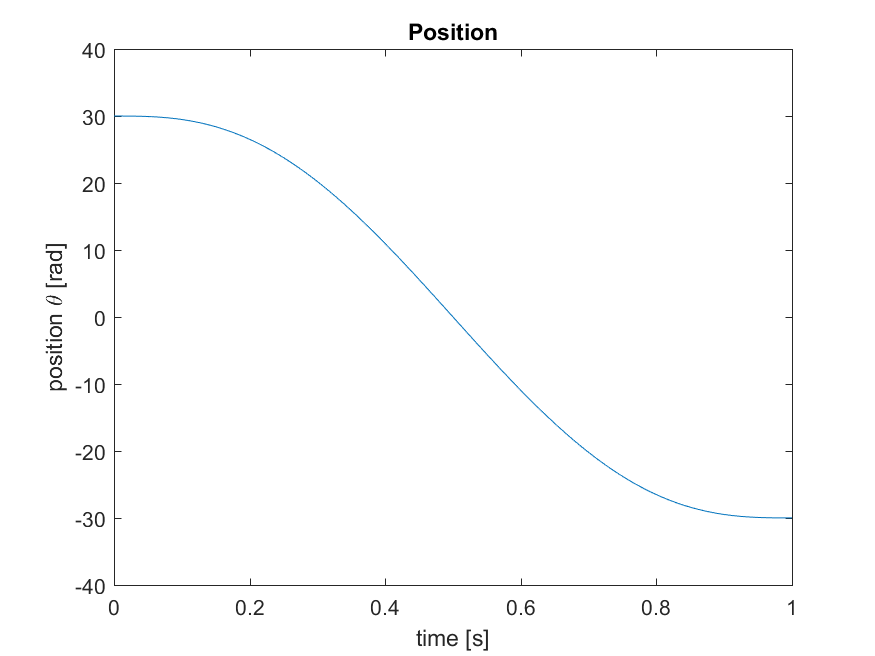
\includegraphics[width=\linewidth]{plot_position}
    \caption{Joint variable normal}
    \label{plot_position}
\end{subfigure}
\hfill
\begin{subfigure}{0.5\textwidth}
    \centering
    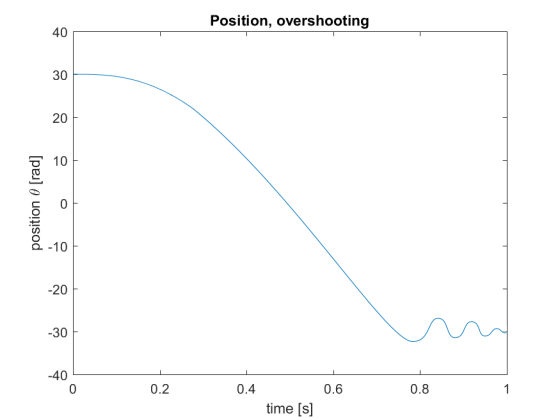
\includegraphics[width=\linewidth]{plot_position_over_edit}
    \caption{Overshooting the wanted joint position}
    \label{plot_position_over}
\end{subfigure}
\caption{Adjusting the joint angle correctly and with an overshoot}
\label{joint_position}
\end{figure}

Another issue arises when the suction cup has to press down on the package. The robot has to press down with sufficient force, but not too much as this could damage the package. Simple moment equations can be used to calculate this for a static situation, but in a situation where the package and/or the robot is moving, the \gls{inforce} has to be accounted for when making these calculations.

\section{Objective}

The goal for this thesis has been to (a), develop a good understanding of the dynamic principles for a serial manipulator, (b) find a suitable algorithm for calculating force and moments in joints because of static and inertial forces and (c) test and verify this algorithm on a robot configuration.

It is important that the chosen algorithm is able to calculate the correct forces for numerous robot configuration. If this is accomplished the calculations will not depend on the type of robot. Any changes made to the robot will therefore not affect the validity of the force and moment calculations.
